\chapter{wxWidgets}
\label{chap:wxWidgets}

{\bf wxWidgets} toolkit (w = Windows, x = X) was created in 1992 as a C++
library, the time when there is no cross-platform open-source widget toolkit
available.
 
\begin{itemize}
  \item to run on Windows, it was first built on top of MFC (Sect.\ref{sec:MFC})
  
Later on, the Windows port was rewritten using native Windows API.
  
  \item to run on Linux, it was first built on top of XView (Sect.\ref{sec:XView})
  
As XView was later abandoned, wxWidgets was rebuilt on top of Motif
(Chap.\ref{chap:Motif}).

In 1995, a Linux port using X toolkit (Sect.\ref{sec:X_toolkit}) was released so
that wxWidgets can run without Motif as Motif was a commercial product at that
time.
  
  \item there is a port using GTK+ (Sect.\ref{sec:GTK+}) called \verb!wxGTK! (Sect.\ref{sec:wxGTk})
  
  \item to run on Linux-based embedded devices, there is a port using DirectFB (Sect.\ref{sec:DirectFB}) called
  \verb!wxDFB! since wxWidgets 3.0 
  
  
\end{itemize}


\url{https://www.wxwidgets.org/about/history/}

\section{wxWidgets}
\label{sec:wxWidgets}

wxWidgets is cross-platform GUI toolkit (LGPL licensed), with binding for Python
(wxPython - Chap.\ref{chap:wxPython}), Perl (wxPerl - Chap.\ref{chap:wxPerl}),
PHP, Java, Lua, Lisp, Erlang, Eiffel, C\#, BASIC, Ruby and Javascript.

% Why not using wxWidgets?
% \begin{itemize}
%   \item Still provide ANSI and Unicode options
%   \item the IDE for wxWidgets is Dev-C++ which has no support for code completion, code generation \ldots 
%   
%   \item wxWidgets does not have an official GUI designer like QT does, however.
%   
%   \item no proxy support in the socket library
%   \item not good documentation
%   \item the design is based on Dev-C++ (a not good IDE)
% \end{itemize}
%   
% Why wxWidgets?
% \begin{itemize}
%   \item cross-platforms
% \end{itemize}

\subsection{Install on Ubuntu}
\label{sec:wxWidgets-install}

\url{http://linuxg.net/how-to-install-wxwidgets-3-0-2-on-ubuntu-14-04-linux-mint-17-elementary-os-0-3-deepin-2014-and-other-ubuntu-14-04-derivatives/}
{\tiny
\begin{verbatim}
sudo apt-key adv --fetch-keys http://repos.codelite.org/CodeLite.asc

sudo apt-add-repository 'deb http://repos.codelite.org/wx3.0.2/ubuntu/ trusty universe'

sudo apt-get update

sudo apt-get install libwxbase3.0-0-unofficial libwxbase3.0-dev libwxgtk3.0-0-unofficial libwxgtk3.0-dev wx3.0-headers wx-common
\end{verbatim}
}


\subsection{Versions 2.x}

As wxWidgets was made to help users that were using MFC to migrate easier, it
inherited a lot of bad things from MFC.

wxWidgets 2.8.6: two separate builds (Unicode \verb!wchar_t*! and ANSI \verb!char*!)

\subsection{Version 3.x}

wxWidgets 3.0 beta: only one build, support Unicode but also support \verb!char *! and
simply convert them using the current encoding transparently.

New classes
\begin{enumerate}
  \item \verb!wxDataViewCtrl! : to replace \verb!wxListCtrl!
\end{enumerate}

Improvements:
\begin{enumerate}
  \item wxFileCtrl 
  \item wxGTK: with wxToolBar, wxStaticText, wxHyperlinkCtrl
  
\end{enumerate}

New features in existing classes
\begin{itemize}
  \item auto-completion: wxTextCtrl and wxComboBox.
\end{itemize}

\url{http://wxwidgets.blogspot.com/2007/11/looking-forward-to-wxwidgets-3.html}

\section{Important classes}

Important classes in wxWidgets toolkit
\begin{enumerate}
  \item \verb!wxSizer! : Sizers are classes derived from the abstract 
  base \verb!wzSizer! class, Fig.\ref{fig:wxSizer_class}
  
\begin{verbatim}
#include <wx/sizer.h>
\end{verbatim}  
  It is a method of choice to define the layout of a control (subwindow) in dialogs (window), 
  as their ability to create a visually appealing
  dialogs independent of the platforms, taking into account the differences in size and 
  style of the individual UI controls.
  
  \url{http://docs.wxwidgets.org/trunk/overview_sizer.html}
  
  The layout algorithm used by sizers in wxWidgets is closely related to layout
  systems in other GUI toolkits, such as Java's AWT, the GTK toolkit or the Qt
  toolkit.
  The idea is that individual subwindows reporting their minimal required size
  and their ability to get stretched if the size of the parent window has
  changed.
\url{http://docs.wxwidgets.org/trunk/classwx_sizer.html}

\begin{figure}[hbt]
  \centerline{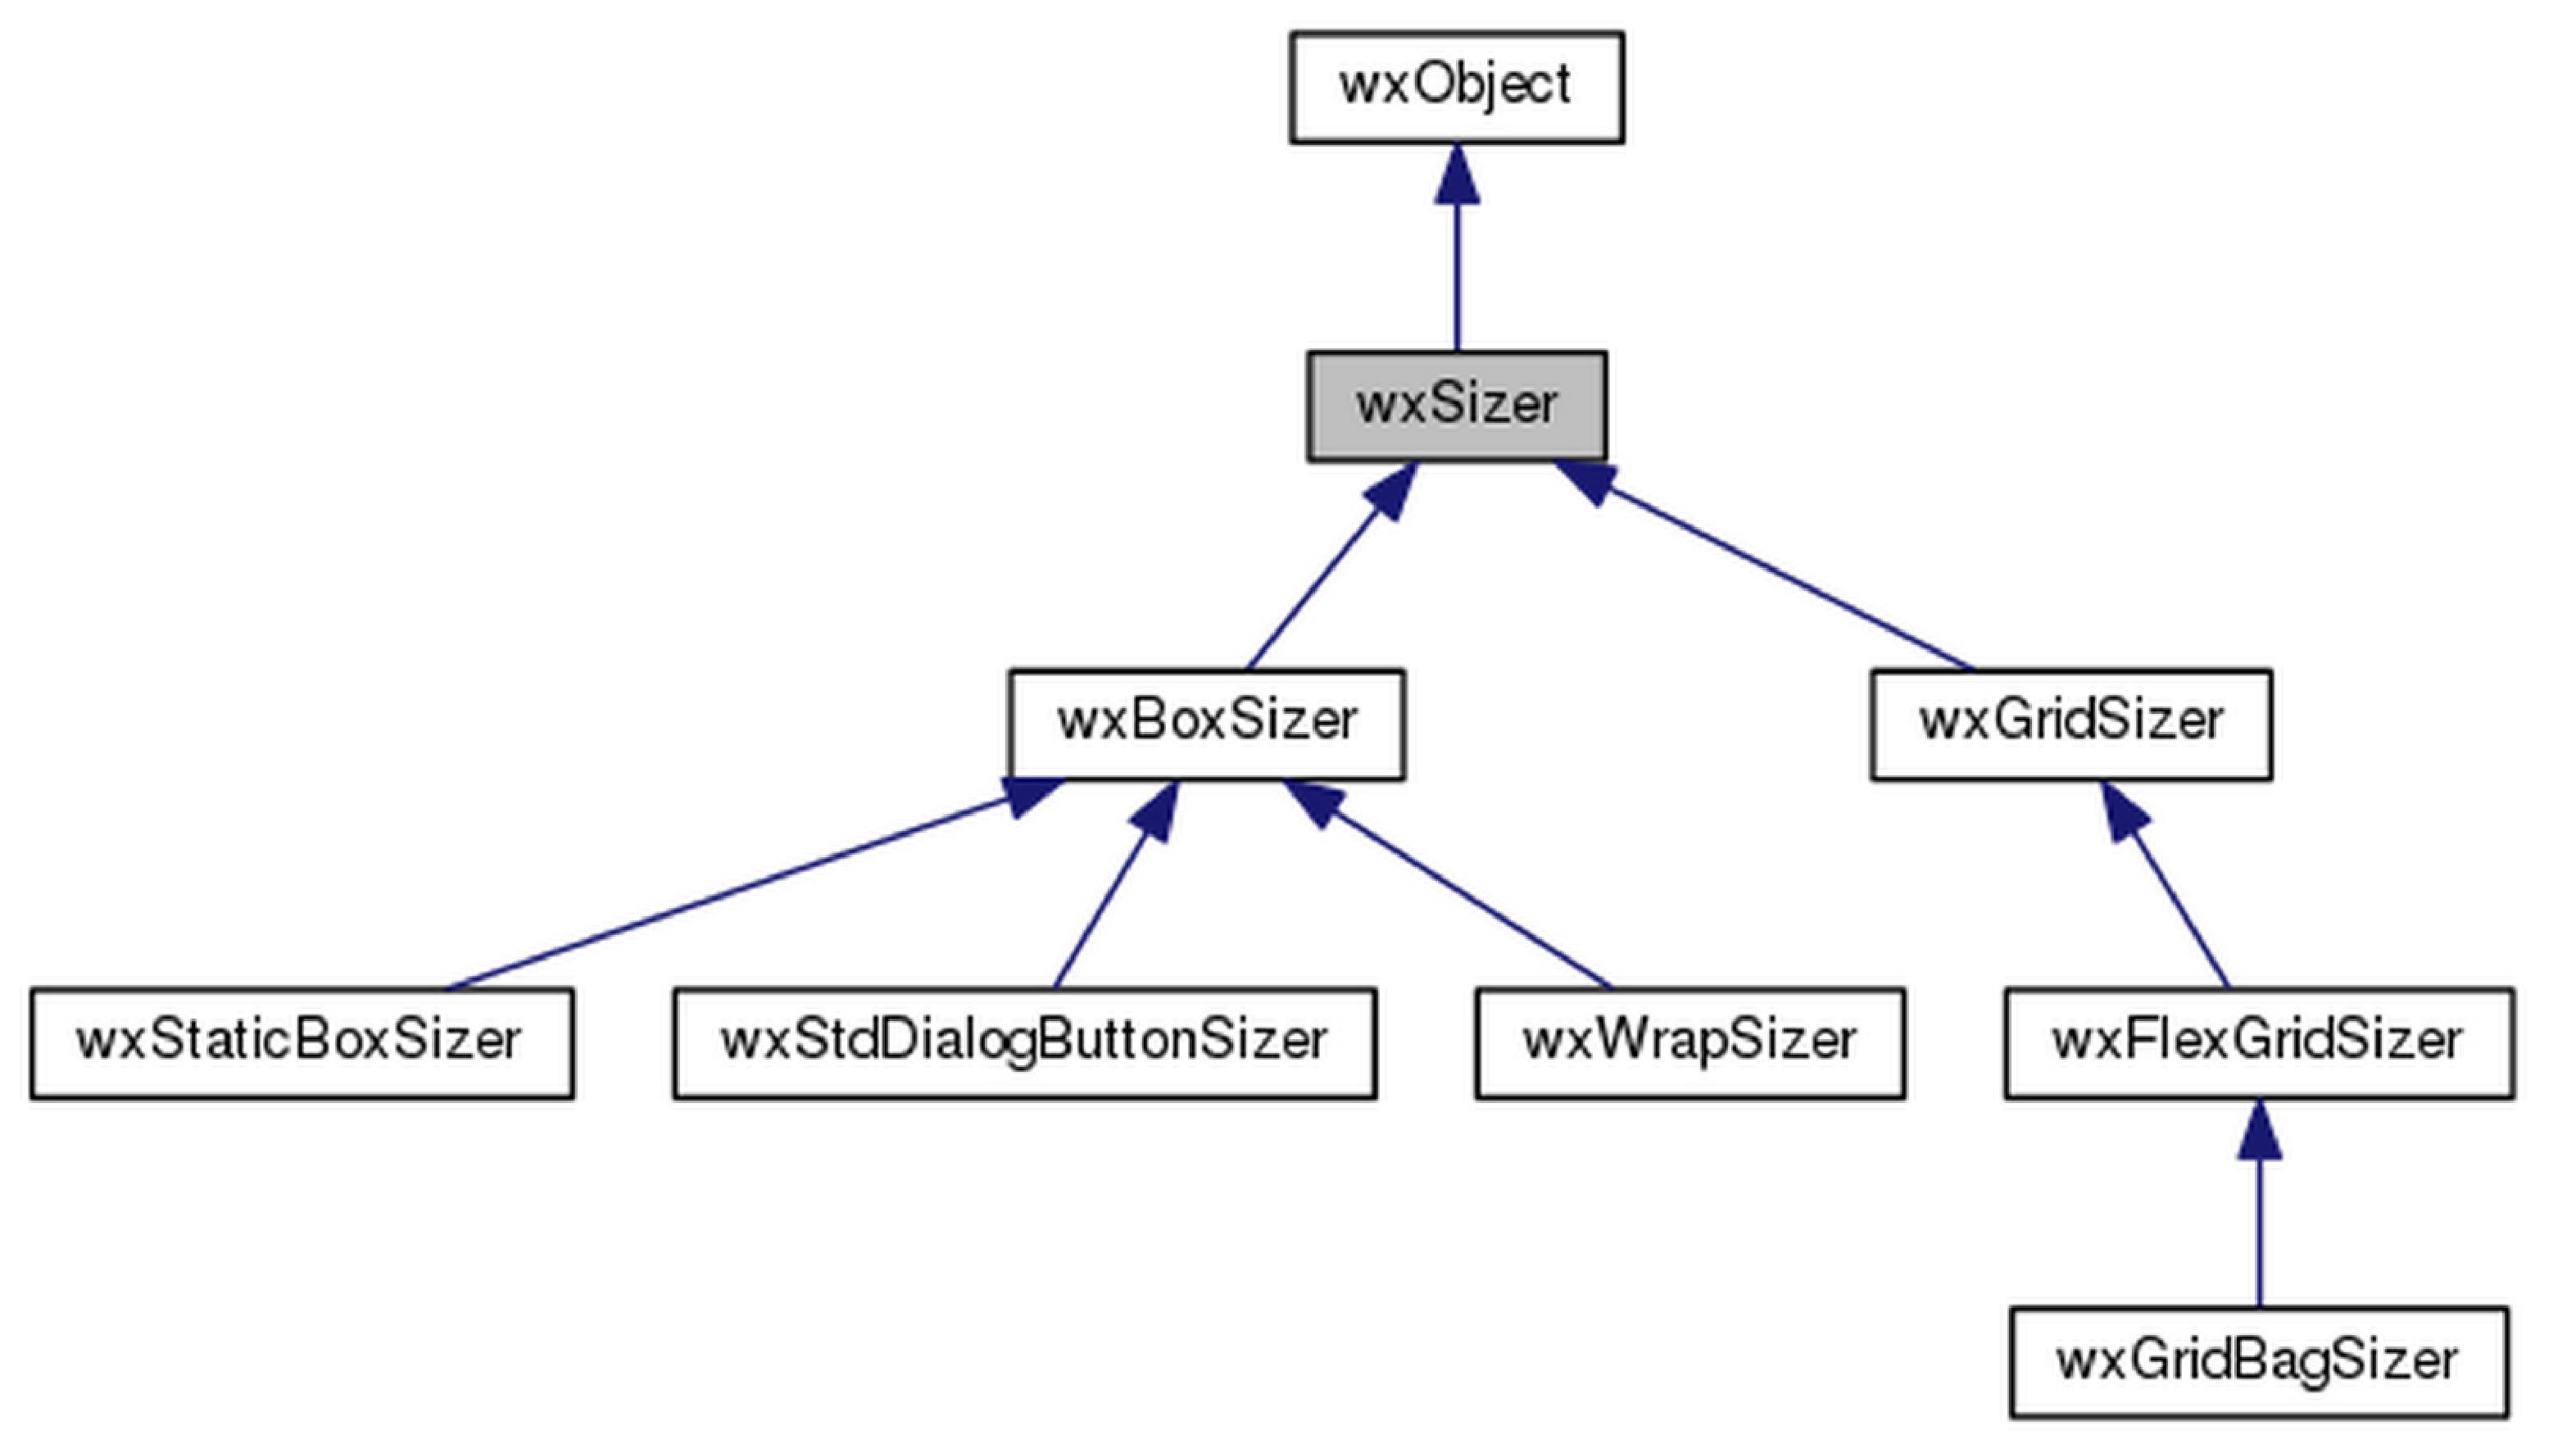
\includegraphics[height=5cm,
    angle=0]{./images/wxSizer_class.eps}}
\caption{wxSizer class hierarchy}
\label{fig:wxSizer_class}
\end{figure}  
  
  
  \item \verb!wxWindow! : a generic class for any drawable object on the screen
  
  \url{http://docs.wxwidgets.org/trunk/classwx_window.html}
  
  \item \verb!wxFrame! (to-level window): A frame is a window whose size and
  position can (usually) be changed by the user, Fig.\ref{fig:wxFrame_class}
  
\begin{verbatim}
#include <wx/frame.h>
\end{verbatim}

It usually has thick borders and a title bar, and can optionally contain a menu
bar, toolbar and status bar. A frame can contain any window that is not a frame
or dialog. 
  
\begin{figure}[hbt]
  \centerline{
\includegraphics[height=5cm,
    angle=0]{./images/wxFrame_class.eps}}
\caption{wxFrame class hierarchy}
\label{fig:wxFrame_class}
\end{figure}  

REMARKS: An application should normally define an wxCloseEvent handler for the
frame to respond to system close events, for example so that related data and
subwindows can be cleaned up.
\url{http://docs.wxwidgets.org/trunk/classwx_frame.html}
    
  \item \verb!wxDialog! : a window for short-term interaction with users to query some information.
  
From the programmer perspective: a dialog does not delete itself after close, so
the information from it can be retrieved it is closed. Thus \verb!wxDialog!
class is often used for preferences dialog (as in web browser) or font dialog
(as in Word processor).

  \item \verb!wxPanel! : a subclass of \verb!wxWindow!. It is a window on which GUI controls are placed.
  
 It is usually placed within a frame (wxFrame).

To have TAB traversal in the frame, we need to use \verb!wxControlContainer! class.
\url{http://docs.wxwidgets.org/trunk/classwx_panel.html}
\begin{verbatim}
#include <wx/containr.h>

#include <wx/panel.h> 
\end{verbatim}

\end{enumerate}


Example: application design: under normal circumstances, you create a frame (subclass of wxFrame),
place a panel in the frame, then place other wxWindow subclasses (wxButton,
wxTextCtrl, etc.) in the panel.



\url{https://wiki.wxwidgets.org/WxFAQ}

\url{https://wiki.wxwidgets.org/Guides_&_Tutorials}


\subsection{wxSizer class}

{\bf wx.BoxSizer} class: and its children
\begin{verbatim}
 wxStaticBoxSizer
 wxStdDialogButtonSizer
 wxWrapSizer
\end{verbatim}

A wx.BoxSizer will lay out its items in a simple row or column, depending on the
orientation parameter passed to the constructor.

It can grow in both directions (height and width) but can distribute its growth
in the main direction (horizontal for a row) unevenly among its children.
 
\url{http://wxpython.org/docs/api/wx.BoxSizer-class.html}




\section{wxGTK library}
\label{sec:wxGTk}

The reason for the existence for wxGTK is to provide a port to using GTK+ via wxWidget. 

However, as there is no static library in GTK+, we can only build linking to GTK+ shared library.

\url{http://stackoverflow.com/questions/1875855/statically-linking-gtk-libaries-in-windows}

\url{https://www.wxwidgets.org/docs/faq/gtk/}

\section{How to write a GUI application with wxWidget?}

A wxWidget application (GUI and console) has no \verb!main()! procedure, 
the reason is that it's not a universal entry point, e.g in Windows \verb!WinMain()! is used.
So, wxWidgets uses the macro \verb!IMPLEMENT_APP(<GUI class>)! as the entry
point, to hide the complexity behind O/S. The equivalent is
\verb!wxApp::OnInit()! member defined in the class derived from \verb!wxApp!.


We need to create an instance of \verb!wxApp! class for a \verb!wxWidget!-based application, 
and implement \verb!__init__! method of this derived class.
If we need the GUI part, inside this method we need to create an instance of
\verb!wxFrame! class, and enable it to show up.

\url{https://wiki.wxwidgets.org/Development:_wxWiki_Documentation_Example}

So for a wxWidget-based GUI application, you need (1) define a subclass of
\verb!wxApp!, (3) call \verb!IMPLEMENT_APP! macro on this derived class, and (3)
implement the \verb!OnInit()! member function of this derived class (with the
minimal implementation is to create a top window) in which we need to create an instance of
\verb!wxFrame! or its derived class.

\begin{verbatim}
#include "wx/wx.h"  // global include

class DerivedApp : public wxApp
{
public:
    virtual bool OnInit();
    
    // define UI controls
    wxCHMHelpController *m_helpCtrl;
};

IMPLEMENT_APP(DerivedApp)

bool DerivedApp::OnInit()
{
  // create the frame, or any UI controls
  
    wxFrame *the_frame = new wxFrame(NULL, ID_MYFRAME, argv[0]);
    ...
    
  // show the frame
    the_frame->Show(true);
    
    // tell which one is the top window
    SetTopWindow(the_frame);

    return true;
}

int MyApp::OnExit()
{
    delete m_helpCtrl;
    return 0;
}
\end{verbatim}
\url{http://packages.das-netzwerkteam.de/doc/wxPython-2.9.1.1/overview_app.html}

Example: define your own frame class, so that you can put more UI controls on it
(Sect.\ref{sec:add_UI_components_to_wxWidget_GUI_Frame})
\begin{verbatim}
class MyFrame: public wxFrame
{
public:
  MyFrame(const wxString& title, const wxPoint& pos, 
                                  const wxSize& size);

  void OnQuit(wxCommandEvent& event);
  void OnAbout(wxCommandEvent& event);

private:
  DECLARE_EVENT_TABLE()
};


\end{verbatim}

\subsection{Building GUI using GUI builder/editor}

To help building the UI faster, we can use widgets Editor for \verb!wxWidgets!
\begin{itemize}
  \item wxWidgets Dialog Editor
  \item wxDesigner
  \item DialogBlocks
  \item XRCed
  \item wxWorkshop
\end{itemize}

\subsection{Working with GUI in multi-threaded application}

wxWidgets (like most GUI toolkits underneath it) is not thread-safe, and
handling of GUI components should always be done exclusively in the main thread.
So your threads must not edit the GUI controls directly, but post an event to
the main thread and let it do the job, i.e.
event passing between thread remains the correct way to go.

\begin{verbatim}
#include <wx/thread.h>
\end{verbatim}

NOTE:  ::wxMutexGuiEnter and ::wxMutexGuiLeave serves as a hack to do the job, but is not recommended.

To send the message, in the form of {\bf custom event}, to the main thread, we follow
\url{https://wiki.wxwidgets.org/Inter-Thread_and_Inter-Process_communication#Sending_custom_events_to_the_main_thread}

\url{http://www.codeproject.com/Articles/11515/Introduction-to-wxWidgets}


\section{How to add menu to Frame}

Define an instance of \verb!wxMenuBar! class. 

To add one or more menu items, define instances of \verb!wxMenu! class
\begin{verbatim}
 menubar = new wxMenuBar;
 file = new wxMenu;
 menubar->Append(file, wxT("&File"));
\end{verbatim}

Finally, set the menu to this instance of \verb!wxMenuBar!
\begin{verbatim}
 SetMenuBar(menubar);
\end{verbatim}

Example: complete

\begin{verbatim}
// absolute.h
#include <wx/wx.h>

class Absolute : public wxFrame
{
public:
  Absolute(const wxString& title);

  wxMenuBar *menubar;
  wxMenu *file;
  wxMenu *edit;
  wxMenu *help;
  wxTextCtrl *textctrl;

};
\end{verbatim}

In the constructor, create the instances of the menu items and assign the text strings
\begin{verbatim}
// absolute.cpp

#include "absolute.h"

Absolute::Absolute(const wxString& title)
       : wxFrame(NULL, -1, title, wxPoint(-1, -1), wxSize(250, 180))
{
 
 wxPanel *panel = new wxPanel(this, -1);

 menubar = new wxMenuBar;
 file = new wxMenu;
 edit = new wxMenu;
 help = new wxMenu;

 menubar->Append(file, wxT("&File"));
 menubar->Append(edit, wxT("&Edit"));
 menubar->Append(help, wxT("&Help"));
 SetMenuBar(menubar);

 textctrl = new wxTextCtrl(panel, -1, wxT(""), wxPoint(-1, -1),
     wxSize(250, 150));

 Centre();
}
\end{verbatim}

Main app
\begin{verbatim}
// main.h
#include <wx/wx.h>

class MyApp : public wxApp
{
  public:
    virtual bool OnInit();
};

// main.cpp
#include "main.h"
#include "absolute.h"

IMPLEMENT_APP(MyApp)

bool MyApp::OnInit()
{

    Absolute *absolute = new Absolute(wxT("Absolute"));
    absolute->Show(true);

    return true;
}
\end{verbatim}

\section{How to add UI components into a Frame}
\label{sec:add_UI_components_to_wxWidget_GUI_Frame}


\section{How to add plots and charts on a GUI application}


There are many add-ons for wxWidgets toolkit 
\begin{itemize}
\item wx"Pl"Plot (another page about this one)
\item wxPlotCtrl (scroll down)
\item wxMathPlot
\item wxChart
\item wxFreeChart
\item gpPanel (another link)
\item wxArt2D
\end{itemize}
\url{https://wiki.wxwidgets.org/WxFAQ#What.27s_the_difference_between_a_wxFrame_and_a_wxWindow.3F} 

\section{How to create a diagram with connected nodes, e.g. a workflow}?

Even though \verb!wxPanel! class is a window on which other UI controls are put on, it is not a good idea 
to create a \verb!wxPanel! for each node.

There are some tools built as an add-on to \verb!wxWidgets!.
The UI controls can be used to help developping workflow workspace,
Fig.\ref{fig:wxShapeFramework_example}

\begin{itemize}
  \item \verb!wxShapeFramework!
  \item \verb!wxWorkspaceView!: tested on wxWidgets 2.8.0 only
  \url{https://code.google.com/p/wxworkspaceview/}
  
  \item \verb!wxArt2D!
\end{itemize}



\begin{figure}[hbt]
  \centerline{\includegraphics[height=5cm,
    angle=0]{./images/wxShapeFramework_example.eps}}
\caption{Examples of GUI applications created using wxShapeFramework}
\label{fig:wxShapeFramework_example}
\end{figure}


\section{How to connect to database}

There is a class called \verb!wxODBC! that helps connecting to different database tools
\begin{verbatim}
  DB2
  DBASE (III, IV)
  Firebird
  Informix
  Interbase
  MaxDB (from MySQL)
  MS Access
  MS SQLServer
  MySQL
  Oracle (7, 8, 9 are tested)
  PervasiveSQL,
  PostgreSQL
  Sybase Adaptive Server Anywhere
  Sybase Adaptive Server Enterprise
  Virtuoso
  XBASE Sequiter
\end{verbatim}
However, \verb!wxODBC! is removed from wxWidgets 2.8.0 and older as no one is maintaining wxODBC.
\url{https://wiki.wxwidgets.org/ODBC}

We can use different database library for database connection. 
\begin{itemize}
  \item SOCI
  
SOCI is a database access library for C++ that makes the illusion of embedding SQL queries in the regular C++ code, staying entirely within the Standard C++.
\url{http://soci.sourceforge.net/}

  \item SQLAPI++:  C++ library for accessing multiple SQL databases (Oracle, SQL Server, DB2, Sybase, Informix, InterBase, SQLBase, MySQL, PostgreSQL, SQLite, SQL Anywhere and ODBC)
  
\url{http://www.sqlapi.com/}

  \item OTL (Oracle and Odbc Template Library):
  
  \url{http://otl.sourceforge.net/} 
\end{itemize}


\section{UI component classes}

\subsection{label}

\verb!wxStaticText! class
\begin{verbatim}

\end{verbatim}

\subsection{generic textbox input}

A text control allows text to be displayed and edited.
The common base class is \verb!wxTextEntry! 
\begin{itemize}
  \item wxTextCtrl: single or multiple-line (with scrollbar)
  
allow text coloring with \verb!wxTE_RICH2! style  
  
  \item wxComboBox: single-line 
  
  \item wxMaskedEditCtrl: limit certain kind of input
  
  \item wxFormatValidator: limit certain kind of input, good for writing localized numbers
\end{itemize}

\url{https://wiki.wxwidgets.org/WxTextCtrl}

\subsection{time  input}

\verb!wxTimePickerCtrl! class allows user to select time. 

\url{http://docs.wxwidgets.org/trunk/classwx_time_picker_ctrl.html}

\subsection{date input}

\verb!wxDatePickerCtrl! class allows user to select date.

\section{Other add-ons libraries}


\begin{verbatim}
wxMozilla.
wxIndustrialControls.
wxCURL.
ToasterBox.
wxVTK.
wxDockIt.
wxIFM.
wxMathPlot.
wxTreeMultiCtrl.
wxAUI.
wxPropertyGrid.
wxSMTP.
wxResizeableControl.
wxOTL.
wxReportWriter.
wxHyperlinkCtrl.
wxSQLite.
wxIE.
wxCTB.
AWX.
wxSpellChecker.
wxArt2D.
wxImprola.
wxHTML.
wxStEdit.
wxLCDWindow.
mmwx.
LitWindow.
Keybinder.
wxBetterDialog.
wxBZipStream.
wxCrashReport.
wxHTTPServer.
wxRarInputStream.
wxSheet.
wxStreamMerger.
\end{verbatim}
\url{http://www.codeproject.com/Articles/11515/Introduction-to-wxWidgets}